\section{Classification}
\label{sec:exp-clf}
    \subsection{Overview}
    \label{subsec:exp-clf-overview}
        In this section, parameters that alter the training set of data-set and those which affect the training process itself will be experimentally optimised to produce near-optimum performance. An exhaustive grid search, without consideration of post-processing, would require training and testing of each classifier approximately $50,000$ times, taking $1000$s of days of computing time. Instead of an exhaustive search, an iterative approach will be taken, depicted in figure \ref{fig:exp-clf-overview-opt}. 
        \newcommand{\optnode}[5]{
    % supernode id, find content, assume content, found content, position 
    \node (#1-find) [smallamber,minimum height=0.1cm ,text width=1.6cm,minimum width = 2cm #5] {\specialcell{#2}};
    \node (#1-assume) [smalldarkbyzantium,minimum height=0.1cm, text width=1.6cm, minimum width = 2cm, below=0.15cm of #1-find] {\specialcell{#3}};
    \node (#1-found) [smallazure,minimum height=0.1cm, text width=1.6cm, minimum width = 2cm, below=0.15cm of #1-assume] {\specialcell{#4}};
    \begin{pgfonlayer}{background}
        \node(#1)[bigblush] [fit = (#1-find) (#1-found)] {};
    \end{pgfonlayer}
}
\def\dist{0.3cm}
\begin{tikzfig}{fig:exp-clf-overview-opt}{Optimisation and iteration of pre-classification pipeline.}{\tiny}
    
    \optnode{feats}{choose features}{balance classes\\normalise audio\\training labels\\classifier params}{normalise features\\testing label}{}
    \optnode{balance}{balance classes}{normalise audio\\training labels\\classifier params}{normalise features\\testing label\\chosen features}{, right=\dist of feats-find}
    \optnode{normaud}{normalise audio}{training labels\\classifier params}{normalise features\\testing label\\chosen features\\balance classes}{, right=\dist of balance-find}
    \optnode{labels}{choose train labels}{classifier params}{normalise features\\testing label\\chosen features\\balance classes\\normalise audio}{, right=\dist of normaud-find}
    \optnode{clf}{classifier params}{none}{normalise features\\testing label\\chosen features\\balance classes\\normalise audio\\chosen train labels}{, right=\dist of labels-find}
    \optnode{done}{none}{none}{normalise features\\testing label\\chosen features\\balance classes\\normalise audio\\chosen train labels\\classifier params}{, right=\dist of clf-find}
    
    \optnode{key}{optimising}{assumed}{chosen/estimated}{, left=3cm of balance-find}

    \draw[arrow](feats)--(balance);
    \draw[arrow](balance)--(normaud);
    \draw[arrow](normaud)--(labels);
    \draw[arrow](labels)--(clf);
    \draw[arrow](clf)--(done);
    \draw [arrow] (done-found.east) -| (12.85,-3.37) |- (-1.4,-3.37)  node[near end,above]{iterate}-| (-1.4,-2) |- (feats-assume.west);

    
\end{tikzfig}
        
        For each stage, one parameter/set of parameters is locally optimised whilst making initial assumptions about the others. The assumed parameters are be sequentially optimised until eventually the whole parameter space has been empirically optimised. These first-iteration optimised parameters are fed back to the start of the pipeline, replacing the initial assumptions and running the procedure until convergence is achieved. This approach means that for each iteration, each classifier will only have to be trained/tested $\sim50$ times. This section is strongly linked with sections \ref{sec:pl-data} to \ref{sec:pl-clf} which detail mathematics and implementations.
        
        Performance will be evaluated using the F1 Score, the area under the ROC curve, the true positive rate (TPR) and the true negative (TNR) rate. These metrics have been chosen as they represent important classifier characteristics in a compact form, convenient for comparing many results. More details regarding metrics can be found in section \ref{sec:pl-test}.
        
    \subsection{Known Parameters}
    \label{subsec:exp-clf-known}  
        \subsubsection{Feature Normalisation}
        \label{subsubsec:exp-clf-known-featnorm}
            Feature normalisation, or \textit{whitening}, is done with reuse of constants for reasons discussed in above and in section \ref{subsec:pl-data-software}. The impact of normalisation depends on the nature of the classifier being used and how similarity/distance is defined. For a random forest classifier, decisions whether to split a node are based on the information/entropy of the feature (discussed further in \ref{subsec:pl-clf-sup}), a criteria that is invariant to monotonic transforms such as feature scaling \cite{Hastie2009}, so normalisation will not be applied for the random forest.
            
            Linear SVM performance, in comparison, is dependent on feature scaline. By not scaling, a feature with larger magnitudes may be assigned a higher importance than one with lower magnitudes. For non-linear kernels, it is dependant on the kernel and how distance/similarity is calculated. Normalisation will be used for the SVM classifier.
            
            Naive Bayes, by design, performs feature scaling when XXXX, \ref{subsec:pl-clf-sup}. 
            
            These conclusions have been confirmed in brief trials where both the random forest and naive Bayes classifiers were unaffected by normalisation, and the SVM was $\sim10$ times slower to train with resultant F1 scores reduced by at least $0.2$.
    
            %[http://stats.stackexchange.com/questions/57010/is-it-essential-to-do-normalization-for-svm-and-random-forest]
        \subsubsection{Testing Labels}
        \label{subsubsec:exp-clf-known-tstlbls}
            \begin{wrapfigure}{r}{0.3\textwidth}
                \centering
                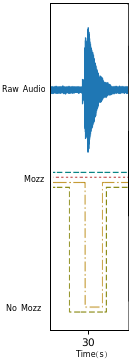
\includegraphics[width=0.2\textwidth]{label_example}
                \caption{An example of talking where there is disagreement between people.}
                \label{fig:exp-clf-known-tstlbls-exmp}
            \end{wrapfigure}
            All the possible training/testing pairs are shown in table \ref{fig:exp-clf-known-tstlbls-tbl}. Although there are $18$ policies in total, it would be incorrect to optimise the pipeline by varying the test labels as this introduces a bias. Instead, where possible, the same aggregation policy should be applied for both training and test labels. Where not possible, i.e. where some samples are rejected for training, a single test label should be chosen. For these experiments, 'consensus\_05\_notmozz' will be selected i.e. a majority vote (at least 3/4) is needed for a positive label. This is based on many areas of the recordings in which there is irregular noise, such as talking, over the sound of a mosquito. Often, two people will class this as positive and two negative, as shown in figure \ref{fig:exp-clf-known-tstlbls-exmp}. In terms of classification, it is desirable to treat this as a negative example to prevent talking being classed as positive, hence why requiring a majority vote is desirable.
            
            \begin{wraptable}{r}{0.58\textwidth}
                \scriptsize
                \singlespacing
                \centering
                    \begin{tabular}{ |l|l|c| } 
                        \hline
                        Train Label & Test Label & Use\\
                        \hline
                        'consensus\_0\_5\_notmozz'&'consensus\_0\_5\_notmozz'& \checkmark \\
                        'consensus\_0\_5\_notmozz'&'consensus\_0\_5\_ismozz'& \xmark\\
                        'consensus\_0\_5\_notmozz'&'sensitive'& \xmark\\
                        'consensus\_0\_5\_ismozz'&'consensus\_0\_5\_ismozz'& \checkmark \\
                        'consensus\_0\_5\_ismozz'&'consensus\_0\_5\_notmozz'& \xmark\\
                        'consensus\_0\_5\_ismozz'&'sensitive'& \xmark\\
                        'sensitive'&'sensitive'& \checkmark\\
                        'sensitive'&'consensus\_0\_5\_notmozz'& \xmark \\
                        'sensitive'&'consensus\_0\_5\_ismozz'& \xmark\\
                        'conf'&'consensus\_0\_5\_notmozz'& \checkmark \\
                        'conf'&'consensus\_0\_5\_ismozz'& \xmark\\
                        'conf'&'sensitive'& \xmark\\
                        '0\_5\_ignore'&'consensus\_0\_5\_notmozz'& \checkmark \\
                        '0\_5\_ignore'&'consensus\_0\_5\_ismozz'& \xmark\\
                        '0\_5\_ignore'&'sensitive'& \xmark\\
                        'multiclass'&'consensus\_0\_5\_notmozz'& \checkmark \\
                        'multiclass'&'consensus\_0\_5\_ismozz'& \xmark\\
                        'multiclass'&'sensitive'& \xmark\\
                        \hline
                    \end{tabular}
                \caption{Training and testing label pairing.}
                \label{fig:exp-clf-known-tstlbls-tbl}
            \end{wraptable}
            
            
    \section{Assumed Parameters}
    \label{subsec:exp-clf-ass}
        \subsubsection{Balanced Classes}
        \label{subsubsec:exp-clf-ass-bal}
            The first assumption made is to balance the classes of the training data. For the Culex \textit{q.} data-set, training data begins with $80024$ and $24695$ samples for classes 0 and 1 respectively, and is balanced to both contain $24695$ samples. Initial experiments have shown this is a sufficient sample size and often leads to better performance and dramatically faster classification times; however, more thorough experimentation will be carried out in this section.
    
        \subsubsection{Audio Normalisation}
        \label{subsubsec:exp-clf-ass-aud}
            The Culex q. data set used has been recorded using the same device in the same location for each of the 57 recordings, therefore mosquitoes flying into and out of the microphone range will have consistent volumes. Some sections of the recordings contain highly irregular noise that is considerably louder than the mosquitoes, an example noisy signal is shown in figure \ref{fig:exp-clf-audio-noisy}.
            \begin{figure}[ht]
                \centering
                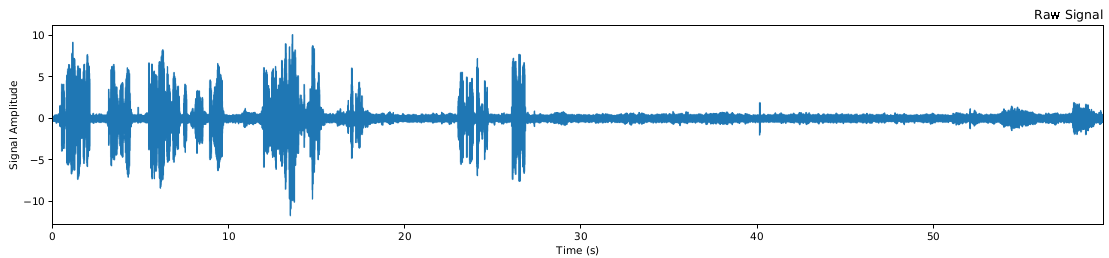
\includegraphics[width=\textwidth]{raw_with_noise}
                \caption{An example of a particularly noisy signal from the Culex. recordings where someone is talking next to the microphone.}
                \label{fig:exp-clf-audio-noisy}
            \end{figure}
            Usually, normalising on a signal-by-signal basis is bad practise for many audio-based machine learning problems due to the time-dependency of the signal as its using information that is 'from the future' for classification, leading to unpredictable consequences. However, this is acceptable in some cases in which the classifier will be used on many samples at a time rather than live sample-by-sample. These acceptable situations include an automated tagging system REF TABLE, a data logger with a buffer REF TABLE or swarm tracking REF TABLE. For on-line applications such as the solar lamp REF or smartphone REF, there is scope for use of more sophisticated algorithms such as Automatic Gain Control (AGC), which has been shown to improve robustness and performance of speech recognition with deep neural networks \cite{Prabhavalkar2015}. However, this will be left for further research due to the complexities of implementation. Both zero-mean and unit-variance normalisation will be assumed at first, then the best performing combination will be determined experimentally. For the on-line case where this is technically incorrect, it will be assumed that a similar level performance could be achieved using an algorithm such as AGC, should normalisation in this way provide better performance than no normalisation. 

        \subsubsection{Training Labels}
        \label{subsubsec:exp-clf-ass-trnlabel}
            \begin{wraptable}{r}{0.4\textwidth}
                \scriptsize
                \singlespacing
                \centering
                    \begin{tabular}{ |c|c|c|c| } 
                        \hline
                        \specialcell{No.\\ Disagreements} & 0 & 1 & 2 \\ 
                        \hline
                        \specialcell{Percentage of \\All Labels} & 77.7\% & 16.2\% & 6.04\% \\ 
                        \hline
                    \end{tabular}
                \caption{Disagreement between four people labelling the same data-set.}
                \label{fig:exp-clf-ass-label-agree}
            \end{wraptable}
            Analysis of these labels, shown in table \ref{fig:exp-clf-ass-label-agree}, emphasises the difficulty of this problem. Of the four people labelling the data, there is only complete agreement $77\%$ of the time, the rest of the time there is at least one person who disagrees with the others.
            Without knowing the details of each persons labelling methodology, a uniform prior must be applied to assign them equal importance for classification use. Therefore, it can be reasoned that it is most appropriate to take a consensus vote to use information from all sets of labels. 
            
            As discussed in section \ref{fig:pl-data-audiolbls-comb}, there are six methods to create a binary consensus label. The 'conf' label set will be assumed initially because it is least likely to contain miss-labelled samples because for a sample to be miss-labelled all four people must get it incorrect. 
            
        \subsubsection{Classifier Parameters}
        \label{subsubsec:exp-clf-ass-param}
            150 trees, rest default
            
        
    \subsection{Optimisation}
    \label{subsec:exp-clf-opt}
    
        \subsubsection{Feature Selection}
        \label{subsubsec:exp-clf-opt-featsel}
            Feature design, as detailed in section \ref{sec:pl-feats}, and selection are crucial to any machine learning problem using traditional classifiers. In order to determine which of the audio features to use, twelve tests will be performed per classifier with the assumed/known parameters specified above. Ten of the tests will be the classifier trained separately on each feature, the other two will be on a feature space that has been dimensionally reduced, one through Recursive Feature Elimination (RFE) and one through Principal Component Analysis (PCA).
            
            \begin{figure}[ht]
                \centering
                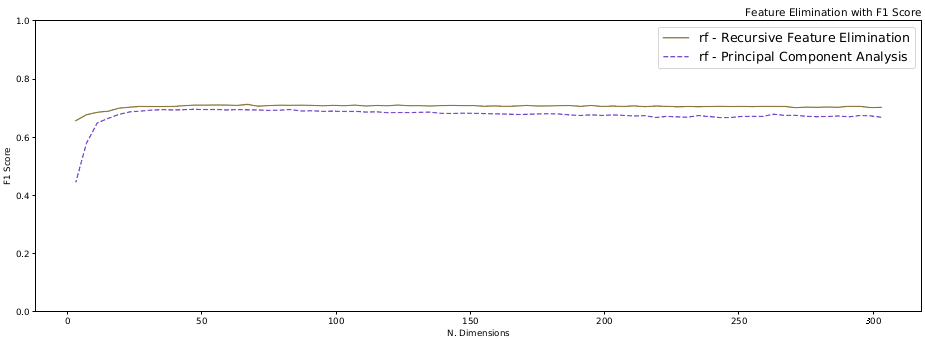
\includegraphics[width=\textwidth]{feature_elim}
                \caption{F1 Score as dimensionality is varied using Recursive Feature Elimination and Principal Component Analysis.}
                \label{fig:exp-clf-opt-featsel}
            \end{figure}
            
            Firstly, suitable degrees of dimensional reduction must be determined. Figure \ref{fig:exp-clf-opt-featsel} shows how the F1 Score for both RFE and PCA are vary with feature-space reduction, generated with a random forest using the methods and reasoning discussed in \ref{subsec:pl-featpreproc-sel}. Similar graphs for ROC area/TPR/TNR show resembling trends. The optimum number of features to eliminate for RFE is around $50$, the indices of the removed features are stored and used to run full analysis on each classifier. PCA shows performance degradation adn will not be considered any further.
            
            %Granitto2006 - original RF-RFE
            %Guyon2002 - original SVM-RFE, more traditional
            
            \begin{wraptable}{r}{0.5\textwidth}
                \scriptsize
                \singlespacing
                \centering
                    \begin{tabular}{ |l|c|c|c|c|c| } 
                        \hline
                        Classifier & Features & F1 & ROC Area & TPR & FPR \\ 
                        \hline
                        NB && $0.$ & $0.$  & $0.$ & $0.$\\
                        NB && $0.$ & $0.$ & $0.$ & $0.$\\
                        NB && $0.$ & $0.$ & $0.$ & $0.$\\
                        \hline
                        RF && $0.$ & $0.$ & $0.$ & $0.$\\
                        RF && $0.$ & $0.$ & $0.$ & $0.$\\
                        RF && $0.$ & $0.$ & $0.$ & $0.$\\
                        \hline
                        SVM && $0.$ & $0.$ & $0.$ & $0.$\\
                        SVM && $0.$ & $0.$ & $0.$ & $0.$\\
                        SVM && $0.$ & $0.$ & $0.$ & $0.$\\
                        \hline
                    \end{tabular}
                \caption{Results of feature selection.}
                \label{fig:exp-clf-opt-feat-res}
            \end{wraptable}
            
            scope for improvement using other methods feat selection, realistically wont improve performance much more, left out of scope of this paper etc etc
            
            Table \ref{fig:exp-clf-opt-feat-res} shows the top three results for each classifier. 
            
            do changing of windows here, say 0.1s res max as that format of lbls
    
    
        \subsubsection{Class Balancing}
        \label{subsubsec:exp-clf-opt-class}
            With the known/assumed parameters set, six experiments are carried out and presented in table \ref{fig:exp-clf-opt-class-res}.
            \begin{wraptable}{r}{0.45\textwidth}
                \scriptsize
                \singlespacing
                \centering
                    \begin{tabular}{ |l|c|c|c|c| } 
                        \hline
                        Classifier & F1 & ROC Area & TPR & FPR \\ 
                        \hline
                        NB          & $0.547$ & $0.715$  & $0.89$ & $0.49$\\
                        NB balanced & $0.547$ & $0.715$ & $0.90$ & $0.49$\\
                        \hline
                        RF          & $0.584$ & $0.852$ & $0.45$ & $0.96$\\
                        RF balanced & $0.661$ & $0.859$ & $0.58$ & $0.93$\\
                        \hline
                        SVM          & $0.608$ & $0.821$ & $0.47$ & $0.98$\\
                        SVM balanced & $0.69$ & $0.843$ & $0.62$ & $0.94$\\
                        \hline
                    
                    \end{tabular}
                \caption{Results of testing balanced training data against non-balanced training data.}
                \label{fig:exp-clf-opt-class-res}
            \end{wraptable}
            In all three cases, classifiers with balanced training data outperform those with imbalanced training data. 
            
            Although overall performance is better, it is interesting to note how balancing classes skews the TPR and TNR to, rather intuitively, increase the former and decrease the latter; a potential technique to tune the classifier at later stages. Further experiments will balance the training data to maximise performance.
        
        \subsubsection{Normalise Audio}
        \label{subsubsec:exp-clf-opt-normaud}
            boop boop
        
        \subsubsection{Label Selection}
        \label{subsubsec:exp-clf-opt-label}
            easy all testies on reduced feature set, multiclass as well
            
        \subsubsection{Classifier Parameters}
        \label{subsubsec:exp-clf-opt-param}
            gini/entropy, svm kernel  - justift keep as linear bc does good enough and nonlinear much longer with probably not much perfomance gain - do a lil test?
            
    \subsection{Iteration}
    \label{subsec:exp-clf-iter}
        just list params that change then list final results




%     start with most detail for random forest, then can tell similar story for the other classifiers in less detail
% Sensors]
%     \subsection{Parameters}
%     \label{subsec:exp-rf-param}
%         \begin{sitemize}
%             \item{start with rf because fast and relatively good results, also gives importance of features}
%             \item{choosing number of trees}
%             \item{decision criterion}
            
%             \item{label selection - binary or mc (binary does better)}
%             \item{postprocessing}
%         \end{sitemize}
    
%     \subsection{Feature Processing}
%     \label{subsec:rf-feats}
%         \begin{sitemize}
%             \item{normalisation (built into sklearn implementation?)}
%             \item{feature selection - shows feature importance as well, do pca and rfe and compare, comment on features picked out as important}
%         \end{sitemize}
    
%     \subsection{Label Selection}
%     \label{subsec:rf-labels}
%         \begin{sitemize}
%             \item{show results with all different labels, binary and multiclass, choose best}
%         \end{sitemize}
        
%     \subsection{Post-Processing}
%     \label{subsec:rf-postproc}
%         \begin{sitemize}
%             \item{show how go from fscore of 0.6ish to 0.75ish}
%             \item{show best for each context, in table}
%         \end{sitemize}